% https://www.overleaf.com/learn

\documentclass{article}
\usepackage{layout}
\usepackage[T1]{fontenc} 
\usepackage[english]{babel}
\usepackage{hyphenat}
\usepackage{graphicx}
\usepackage{listings}
\usepackage{xcolor}
\usepackage{hyperref}

\hypersetup{
    colorlinks=true,
    linkcolor=blue,
    filecolor=magenta,      
    urlcolor=cyan
    }

\usepackage{geometry}
\setlength{\textheight}{640pt}
\geometry{
  a4paper,
  % total={170mm,257mm},
  % left=20mm,
  top=30mm,
  bottom=30mm,
}
\definecolor{codegreen}{rgb}{0,0.6,0}
\definecolor{codegray}{rgb}{0.5,0.5,0.5}
\definecolor{codepurple}{rgb}{0.58,0,0.82}
\definecolor{backcolour}{rgb}{0.95,0.95,0.92}

\lstdefinestyle{mystyle}{
    backgroundcolor=\color{backcolour},   
    commentstyle=\color{codegreen},
    keywordstyle=\color{magenta},
    numberstyle=\tiny\color{codegray},
    stringstyle=\color{codepurple},
    basicstyle=\ttfamily\footnotesize,
    breakatwhitespace=false,         
    breaklines=true,                 
    captionpos=b,                    
    keepspaces=true,                 
    numbers=left,                    
    numbersep=5pt,                  
    showspaces=false,                
    showstringspaces=false,
    showtabs=false,                  
    tabsize=2
}

\title{Project Exam Algorithmic Game Theory}
\author{Paola Guarasci --- mat 231847}
\date{\today}
\lstset{style=mystyle}

% \hyphenation{mate-mati-ca recu-perare}

\begin{document}
\maketitle

%%%%%%%%%%%%%%%%%%%%%%
%%%  Prima parte  %%%%
%%%%%%%%%%%%%%%%%%%%%%

\section*{Description}
\paragraph*{Initial scenario}
The problem concerns the selection of a subset of users within a larger group of users who will have to tour between certain cities. Furthermore, it is necessary to establish the cost to be charged to each user.
\paragraph*{Input}
The input algorithm expects a list of types, one for each user. The type represents each agent's preferred location. A simplification has been introduced regarding the problem originally posed: agents do not provide a list of preferences but a single preference that can be trusted since a choice mechanism based on the maximum payment that each agent is willing to make has been adopted. Therefore, since the payment affirmation can be trusted, it was then decided to use this criterion as a discriminant as regards the inclusion of the single agent in the traveler subset, that is, the set of travelers.
In the algorithm testing phase, the input was generated randomly, respecting the cardinality limits of the set of locations (no agent can prefer a location that does not exist).
\paragraph*{Graph}
Locations are represented by an undirected weighted graph. Each locality, that is, each node, is connected with all the other localities. The weights on the arches indicate the distance in kilometers between the two nodes at the ends of each arch.
\begin{figure}[h]
  \centering
  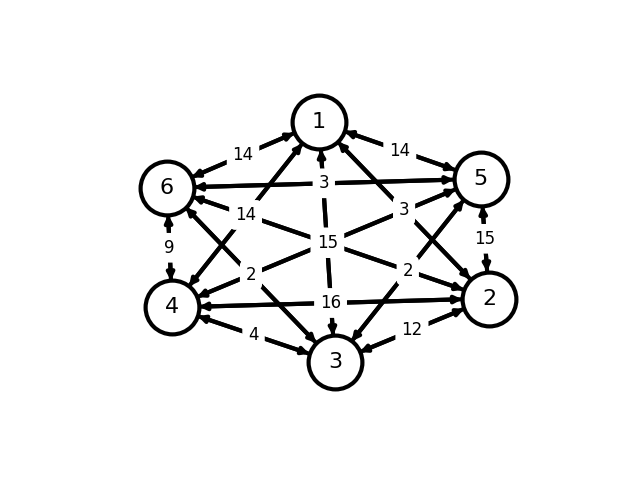
\includegraphics[width=0.50\textwidth]{img/graphTot.png}
  \caption{General graph of the localities}\label{fig:graphTot.png}
\end{figure}
The calculation of the optimal route and its cost was modeled using Dijkstra's algorithm and solving the Traveling Salesman problem. To do this we used an excellent Python library for graph manipulation\footnote{NetworkX, released under BSD license (Open Source) \url{https://networkx.org/}}. The library function \verb|approx.greedy_tsp(graph)| it takes a graph (or portion of it) as input and calculates its Hemiltonian path.
To get the cost of the travel, the formula used is the following:
\begin{lstlisting}[language=Python]
cost = sum(graph[n][nbr]["weight"] for n, nbr in nx.utils.pairwise(cycle))
\end{lstlisting}
The graph is modeled as a list of edge tuples with three values: starting node, ending node, weight.
The nodes are inferred from the list of edges.
\paragraph*{Output}
On output you get a list of travelers and a list of selected locations.
\paragraph*{Mechanism}
The core of the project is the agent selection algorithm. For each agent, the possibility of inclusion in the group of travelers, the \ verb | travelers |, is evaluated using the following selection strategy:
\begin{itemize}
  \item If the maximum capacity of the machine has been reached, do nothing.
  \item Otherwise, evaluate the cost of travel between the locations already selected and the new one preferred by the agent.
  \item If the cost is acceptable and the constraints in terms of maximum kilometers are not exceeded, then enter the agent in the traveler group and the new location in the selected location group.
  \item Finally, for each user already included in the travelers group, it evaluates whether the new cost of the trip is acceptable and if it should not be, it eliminates the agent from the travelers group. Also delete the chosen location if it is not preferred by any agent remaining in the traveler group.
\end{itemize}
It is a direct mechanism whose method of selecting each individual traveler allows you to be sure about the application of dominant strategies by the various agents, since it does not take place through utilities, which by definition (see trace) is not reliable, but occurs in based on the payment that each agent is willing to make (considered reliable).
The fixed cost for each agent is calculated by dividing the sum by the cardinality of the set \verb|travellers|.
\paragraph*{Example of output}
Here is an example output: the first line is the selected users, the second line is the selected locations, then the total travel cost and per capita travel cost.
\begin{lstlisting}[language=bash]
$ python src/agt.py
Travellers:  {(2, 98, 13), (5, 93, 24), (4, 51, 23), (2, 10, 21), (1, 84, 24)}
Locations:  {1, 2, 4, 5}
Num Travellers:  5
Travel cost:  54.0
Travel cost for each user:  12.8
\end{lstlisting}

\begin{figure}[h]
  \centering
  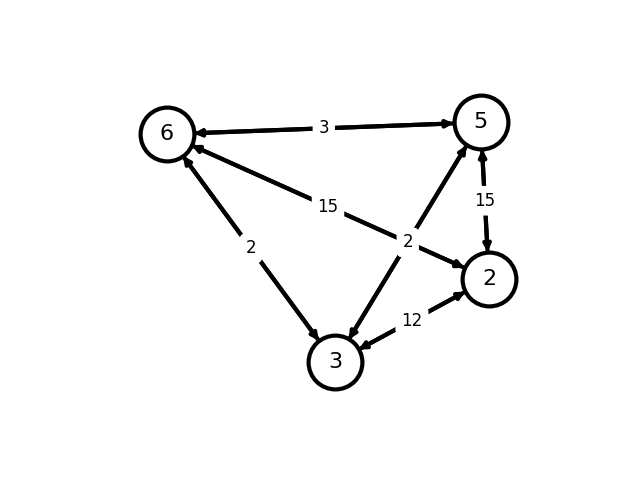
\includegraphics[width=0.50\textwidth]{img/graphOutput.png}
  \caption{Sub-graph with locations selected for the tour}\label{fig:graphOutput.png}
\end{figure}
\clearpage
\pagebreak

%%%%%%%%%%%%%%%%%%%%%%
%%% Seconda parte %%%%
%%%%%%%%%%%%%%%%%%%%%%

\section*{Implementation}
\lstinputlisting[language=Python]{../src/agt.py}
\end{document}